\section{弱大数律}
\label{sec:lln-weak-law}

现在把部分和除以$n$。设$X_1,X_2,\dots$独立同分布，共同的均值为$\mu$。在一个固定的样本量$n$下，样本平均$\bar{X}_n$偏离$\mu$超过给定精度的机会有多大，它是否随$n$增大而趋于零？用第~\ref{chap:random-variable-convergence}章的语言，问题是$\bar{X}_n$是否依概率收敛到$\mu$。

\begin{definition}[弱大数律]
\label{def:lln-weak-law}
设随机变量列$X_1,X_2,\dots$各项可积且有共同的均值$\mu$。若$\bar{X}_n\xrightarrow{\mathbb{P}}\mu$，即对每个$\varepsilon>0$，
\begin{equation}
 \lim_{n\to\infty}\mathbb{P}\bigl(\lvert\bar{X}_n-\mu\rvert\geq\varepsilon\bigr)=0 ,
 \label{eq:lln-weak-law}
\end{equation}
则称这列变量满足\term{弱大数律}（weak law of large numbers）。
\end{definition}

“平均把波动抹平”是这里的直观：每个观测的偏差有正有负，平均以后互相抵消，剩余的偏差随$n$缩小。两种情形用到的抹平机制不同。有限方差时，方差按$1/n$缩小，一步即得；只有一阶矩时，偶尔出现的大值不能用方差衡量，需要先截断。

\subsection{有限方差情形}
\label{sec:lln-wlln-variance}

方差有限时，式~\eqref{eq:lln-sum-variance}已经给出$\operatorname{Var}(\bar{X}_n)$，再用Chebyshev不等式就够了。下面的陈述把独立同分布放宽到实际用到的条件。

\begin{theorem}[有限方差的弱大数律]
\label{thm:lln-wlln-variance}
设$X_1,\dots,X_n$两两不相关，有共同的均值$\mu$，且$\operatorname{Var}(X_k)\leq\sigma^2<\infty$。则对每个$\varepsilon>0$，
\begin{equation}
 \mathbb{E}\bigl[(\bar{X}_n-\mu)^2\bigr]\leq\frac{\sigma^2}{n},\qquad
 \mathbb{P}\bigl(\lvert\bar{X}_n-\mu\rvert\geq\varepsilon\bigr)\leq\frac{\sigma^2}{n\varepsilon^2} .
 \label{eq:lln-wlln-chebyshev}
\end{equation}
特别地，独立同分布且方差有限的序列满足弱大数律，并且$\bar{X}_n\xrightarrow{L^{2}}\mu$。
\end{theorem}

\begin{proof}
$\mathbb{E}[\bar{X}_n]=\mu$。由式~\eqref{eq:lln-sum-variance}（它只用了两两不相关），
\[
 \mathbb{E}\bigl[(\bar{X}_n-\mu)^2\bigr]=\operatorname{Var}(\bar{X}_n)=\frac{1}{n^2}\sum_{k=1}^{n}\operatorname{Var}(X_k)\leq\frac{n\sigma^2}{n^2}=\frac{\sigma^2}{n} .
\]
对$\bar{X}_n$用第~\ref{chap:tail-probabilities}章的Chebyshev不等式，就得到第二个不等式。右边随$n\to\infty$趋于零。
\end{proof}

\paragraph{读懂这个上界}
式~\eqref{eq:lln-wlln-chebyshev}中三个量各有含义。$\sigma^2$是单个观测的分散程度，越分散需要越多观测；$n$出现在分母上，是平均带来的抹平；$\varepsilon^2$表示精度的代价，要求精度提高一倍，样本量就要增加到四倍。反过来，要使偏差概率不超过$\delta$，只要
\[
 n\geq\frac{\sigma^2}{\delta\varepsilon^2} .
\]
这是一个有限样本的保证：对每个具体的$n$都成立，不是只在极限中成立。

\paragraph{两个例子}
掷均匀硬币，$X_k\sim\operatorname{Bern}(1/2)$，$\sigma^2=1/4$。取$\varepsilon=0.05$，式~\eqref{eq:lln-wlln-chebyshev}给出
\[
 \mathbb{P}\bigl(\lvert\bar{X}_n-0.5\rvert\geq0.05\bigr)\leq\frac{1/4}{n\cdot0.0025}=\frac{100}{n} .
\]
$n=400$时界为$0.25$。由二项分布直接求和，精确值是$0.0510$。

掷均匀骰子，$\sigma^2=35/12$。取$\varepsilon=0.1$，界为
\[
 \mathbb{P}\bigl(\lvert\bar{X}_n-3.5\rvert\geq0.1\bigr)\leq\frac{35/12}{0.01\,n}\approx\frac{291.7}{n} ,
\]
$n=10^4$时不超过$0.0292$。

图~\ref{fig:lln-wlln-chebyshev}在对数坐标中比较硬币例子的精确概率与界。界按$1/n$下降，精确值在$n$大时下降得快得多：$n=1000$时精确值约为$0.0016$，界为$0.1$。差距的原因是Chebyshev不等式只用了方差。对有界变量，第~\ref{chap:tail-probabilities}章的指数矩方法能给出随$n$指数衰减的界；这里关心的是收敛本身，方差已经足够。

\begin{BookInlineFigure}
 \centering
 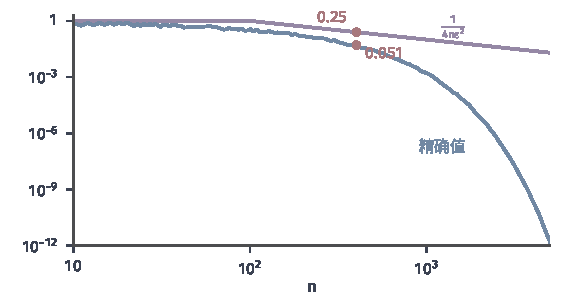
\includegraphics[width=96mm]{figures/07-probability/03-probability-limits/matplotlib/lln-wlln-chebyshev/figure.pdf}
 \caption{均匀硬币的频率偏离$1/2$至少$0.05$的概率，双对数坐标。蓝线为二项分布的精确值，紫线为Chebyshev界$\min\{1,1/(4n\varepsilon^2)\}$，$\varepsilon=0.05$；红点标出$n=400$处的两个值。}
 \label{fig:lln-wlln-chebyshev}
\end{BookInlineFigure}

\paragraph{速度依赖二阶矩}
式~\eqref{eq:lln-wlln-chebyshev}的$1/n$速度来自方差有限这一假设。只知道一阶矩有限时，Chebyshev不等式无法使用，一般也得不到这样的速度：下一小节的Pareto例子中，样本平均的路径时有大的跳跃，靠近均值的过程明显更慢。

\subsection{可积情形}
\label{sec:lln-wlln-integrable}

很多分布均值有限而方差无穷。第~\ref{chap:tail-probabilities}章的Pareto分布，密度为$\alpha x^{-\alpha-1}$（$x\geq1$），取$\alpha=1.5$时
\[
 \mathbb{E}[X]=\int_1^{\infty}x\cdot1.5x^{-2.5}\,\mathrm{d}x=3,\qquad \mathbb{E}[X^2]=\int_1^{\infty}1.5x^{-0.5}\,\mathrm{d}x=\infty .
\]
这时$\operatorname{Var}(\bar{X}_n)=\infty$，Chebyshev不等式无从下手。平均仍应抹平波动，困难在于偶尔出现的大值。办法是先截断：截断后的部分有界，可以用上一小节；被截掉的部分出现得少，用一阶矩控制。

\begin{theorem}[可积情形的弱大数律]
\label{thm:lln-wlln-integrable}
设$X_1,X_2,\dots$独立同分布，$\mathbb{E}[\lvert X_1\rvert]<\infty$，$\mu=\mathbb{E}[X_1]$。则$\bar{X}_n\xrightarrow{\mathbb{P}}\mu$。
\end{theorem}

\begin{proof}
固定$c>0$，把每项分成截断部分与被截掉的部分：
\[
 Y_k=X_k\mathbf{1}_{\{\lvert X_k\rvert\leq c\}},\qquad Z_k=X_k-Y_k=X_k\mathbf{1}_{\{\lvert X_k\rvert>c\}} ,
\]
并记
\[
 \mu_c=\mathbb{E}[Y_1],\qquad \tau(c)=\mathbb{E}\bigl[\lvert X_1\rvert\mathbf{1}_{\{\lvert X_1\rvert>c\}}\bigr]=\mathbb{E}[\lvert Z_1\rvert] .
\]
$\tau(c)$是截掉部分的平均大小。由$\mu=\mu_c+\mathbb{E}[Z_1]$，样本平均的偏差拆成三项：
\[
 \bar{X}_n-\mu=\bigl(\bar{Y}_n-\mu_c\bigr)+\bar{Z}_n-\mathbb{E}[Z_1] ,
\]
其中$\bar{Y}_n$、$\bar{Z}_n$是$Y_k$、$Z_k$的平均。最后一项满足$\lvert\mathbb{E}[Z_1]\rvert\leq\tau(c)$。

固定$\varepsilon>0$，并先假设$c$足够大，使$\tau(c)<\varepsilon/3$。若$\lvert\bar{X}_n-\mu\rvert\geq\varepsilon$，则前两项中至少有一项的绝对值不小于$\varepsilon/3$，所以
\[
 \mathbb{P}\bigl(\lvert\bar{X}_n-\mu\rvert\geq\varepsilon\bigr)\leq\mathbb{P}\bigl(\lvert\bar{Y}_n-\mu_c\rvert\geq\tfrac{\varepsilon}{3}\bigr)+\mathbb{P}\bigl(\lvert\bar{Z}_n\rvert\geq\tfrac{\varepsilon}{3}\bigr) .
\]

第一项是有界变量的平均。$Y_k$独立同分布，且$\lvert Y_1\rvert\leq c$，所以
\[
 \operatorname{Var}(Y_1)\leq\mathbb{E}[Y_1^2]\leq c\,\mathbb{E}[\lvert Y_1\rvert]\leq c\,\mathbb{E}[\lvert X_1\rvert] .
\]
由定理~\ref{thm:lln-wlln-variance}，第一项不超过$9c\,\mathbb{E}[\lvert X_1\rvert]/(n\varepsilon^2)$。第二项用Markov不等式。由三角不等式与同分布，
\[
 \mathbb{E}\bigl[\lvert\bar{Z}_n\rvert\bigr]\leq\frac1n\sum_{k=1}^{n}\mathbb{E}\bigl[\lvert Z_k\rvert\bigr]=\tau(c) ,
\]
所以第二项不超过$3\tau(c)/\varepsilon$。合起来，
\begin{equation}
 \mathbb{P}\bigl(\lvert\bar{X}_n-\mu\rvert\geq\varepsilon\bigr)\leq\frac{9c\,\mathbb{E}[\lvert X_1\rvert]}{n\varepsilon^2}+\frac{3\tau(c)}{\varepsilon} .
 \label{eq:lln-wlln-truncation-bound}
\end{equation}

现在按顺序取极限。先固定$c$令$n\to\infty$，第一项趋于零，得到
\[
 \limsup_{n\to\infty}\mathbb{P}\bigl(\lvert\bar{X}_n-\mu\rvert\geq\varepsilon\bigr)\leq\frac{3\tau(c)}{\varepsilon} .
\]
左边与$c$无关。再令$c\to\infty$：$\lvert X_1\rvert\mathbf{1}_{\{\lvert X_1\rvert>c\}}$逐点趋于零，且被可积的$\lvert X_1\rvert$控制，由支配收敛定理$\tau(c)\to0$。所以左边的上极限为零。
\end{proof}

\paragraph{两个极限的顺序}
式~\eqref{eq:lln-wlln-truncation-bound}的两项此消彼长。截断水平$c$越高，被截掉的部分越小，第二项越小；但留下的部分取值范围越宽，第一项越大。对固定的$n$，令$c\to\infty$会使第一项发散，所以必须先让$n$增大，再放大$c$。等价地说，有用的截断水平要随样本量一起增长，但增长得比$n$慢。

用$\alpha=1.5$的Pareto分布具体看这种权衡。截掉部分的平均大小为
\[
 \tau(c)=\int_c^{\infty}x\cdot1.5x^{-2.5}\,\mathrm{d}x=3c^{-1/2},\qquad c\geq1 ,
\]
截断变量的二阶矩也可以精确算出，
\[
 \mathbb{E}[Y_1^2]=\int_1^c x^2\cdot1.5x^{-2.5}\,\mathrm{d}x=3(\sqrt{c}-1) ,
\]
比证明中用的$c\,\mathbb{E}[X_1]=3c$小得多。取$\varepsilon=1$，用精确的二阶矩代替$c\,\mathbb{E}[\lvert X_1\rvert]$，上界成为
\[
 \frac{27(\sqrt{c}-1)}{n}+\frac{9}{\sqrt{c}},\qquad c>81 ,
\]
其中$c>81$保证$\tau(c)<1/3$。

图~\ref{fig:lln-truncation-tradeoff}(a)画出被截掉的部分：曲线$xf(x)$下$c$右侧的面积就是$\tau(c)$。图(b)画出不同$n$下的总上界。$n=10^4$时最佳截断约为$c\approx3.4\times10^3$，上界约为$0.31$；$n=10^6$时最佳截断移到$c\approx3.3\times10^5$，上界降到约$0.031$。最佳截断水平随$n$增长，上界随之下降。

\begin{BookInlineFigure}
 \centering
 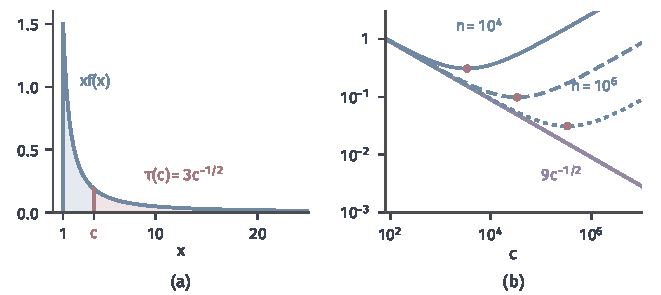
\includegraphics[width=112mm]{figures/07-probability/03-probability-limits/matplotlib/lln-truncation-tradeoff/figure.pdf}
 \caption{$\alpha=1.5$的Pareto分布在弱大数律证明中的截断权衡。(a)求均值的被积函数$xf(x)=1.5x^{-1.5}$（蓝线），截断水平$c=4$左侧为保留部分（浅蓝），右侧为截掉部分（浅红），右侧面积为$\tau(4)=1.5$；(b)$\varepsilon=1$时的上界$27(\sqrt{c}-1)/n+9c^{-1/2}$，蓝色实线、虚线、点线分别对应$n=10^4,10^5,10^6$，红点为各自的最小值，紫线为与$n$无关的第二项$9c^{-1/2}$，双对数坐标。}
 \label{fig:lln-truncation-tradeoff}
\end{BookInlineFigure}

\paragraph{平均意义下的收敛}
同一个截断论证还给出$L^1$收敛。由三角不等式，并对$W=\bar{Y}_n-\mu_c$用一阶绝对矩不超过二阶矩的平方根，
\[
 \mathbb{E}\bigl[\lvert\bar{X}_n-\mu\rvert\bigr]\leq\sqrt{\operatorname{Var}(\bar{Y}_n)}+\mathbb{E}[\lvert\bar{Z}_n\rvert]+\tau(c)\leq\sqrt{\frac{c\,\mathbb{E}[\lvert X_1\rvert]}{n}}+2\tau(c) .
\]
同样先令$n\to\infty$再令$c\to\infty$，得到$\bar{X}_n\xrightarrow{L^{1}}\mu$。

\paragraph{可积不是有限方差}
定理只要求$\mathbb{E}[\lvert X_1\rvert]<\infty$。图~\ref{fig:lln-pareto-cauchy}(a)是$\alpha=1.5$的Pareto样本平均：五条路径最终都靠近$\mu=3$，但不时被一个大观测猛地抬高，再慢慢回落。$n=10^5$时五个平均分别约为$3.00$、$2.98$、$2.97$、$2.97$、$2.92$，多数略低于$3$，因为把平均拉回$3$的正是那些尚未出现的稀有大值。

如果连一阶矩都没有，平均就不再稳定。图(b)是标准Cauchy分布的样本平均，路径不断被新的极端值拉到别处。第~\ref{chap:weak-convergence-of-distributions}章用特征函数可以证明，独立标准Cauchy变量的平均$\bar{X}_n$对每个$n$仍服从标准Cauchy分布，于是
\[
 \mathbb{P}\bigl(\lvert\bar{X}_n\rvert\geq1\bigr)=1-\frac{2}{\pi}\arctan1=\frac12\quad\text{对所有}\ n ,
\]
不趋于零。平均$n$个观测与只看一个观测效果相同，抹平机制完全失效。

\begin{BookInlineFigure}
 \centering
 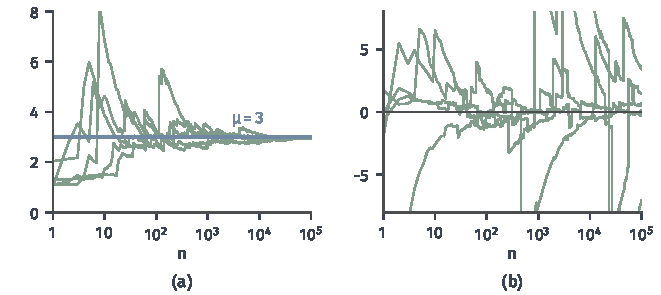
\includegraphics[width=112mm]{figures/07-probability/03-probability-limits/matplotlib/lln-pareto-cauchy/figure.pdf}
 \caption{重尾样本的平均，每图五条路径，横轴为对数刻度。(a)$\alpha=1.5$的Pareto分布（种子$13$），均值$\mu=3$（蓝线），方差无穷；(b)标准Cauchy分布（种子$14$），均值不存在，纵轴截在$[-8,8]$。}
 \label{fig:lln-pareto-cauchy}
\end{BookInlineFigure}
